\chapter{Thiết kế giải pháp và quy trình học máy}
\section{Quy trình tổng quát}
Nhóm em triển khai theo các bước: đọc ảnh và nhãn; kiểm tra metadata và split; tiền xử lý ảnh; trích xuất đặc trưng; huấn luyện các cấu hình trên train; so sánh bằng validation; cuối cùng lưu cấu hình, chỉ số và hình phân tích. Toàn bộ pipeline được xây dựng dựa trên các thư viện mã nguồn mở chuẩn mực gồm scikit-learn \cite{sklearn} và scikit-image \cite{skimage}. Việc tổ chức theo các bước giúp nhóm có thể kiểm tra một phần riêng mà không cần viết lại toàn bộ quy trình.

Hình \ref{fig:pipelinesodo} minh họa toàn bộ quy trình từ dữ liệu thô đến đánh giá và phân tích lỗi. Sơ đồ làm nổi bật ranh giới chống rò rỉ dữ liệu (leak-free boundary): trong giai đoạn chọn cấu hình, PCA chỉ được fit trên train hoặc fold train. Ở lần test đã thực hiện, PCA được fit lại trên train+validation sau lựa chọn; test không tham gia fit.
\begin{figure}[htbp]\centering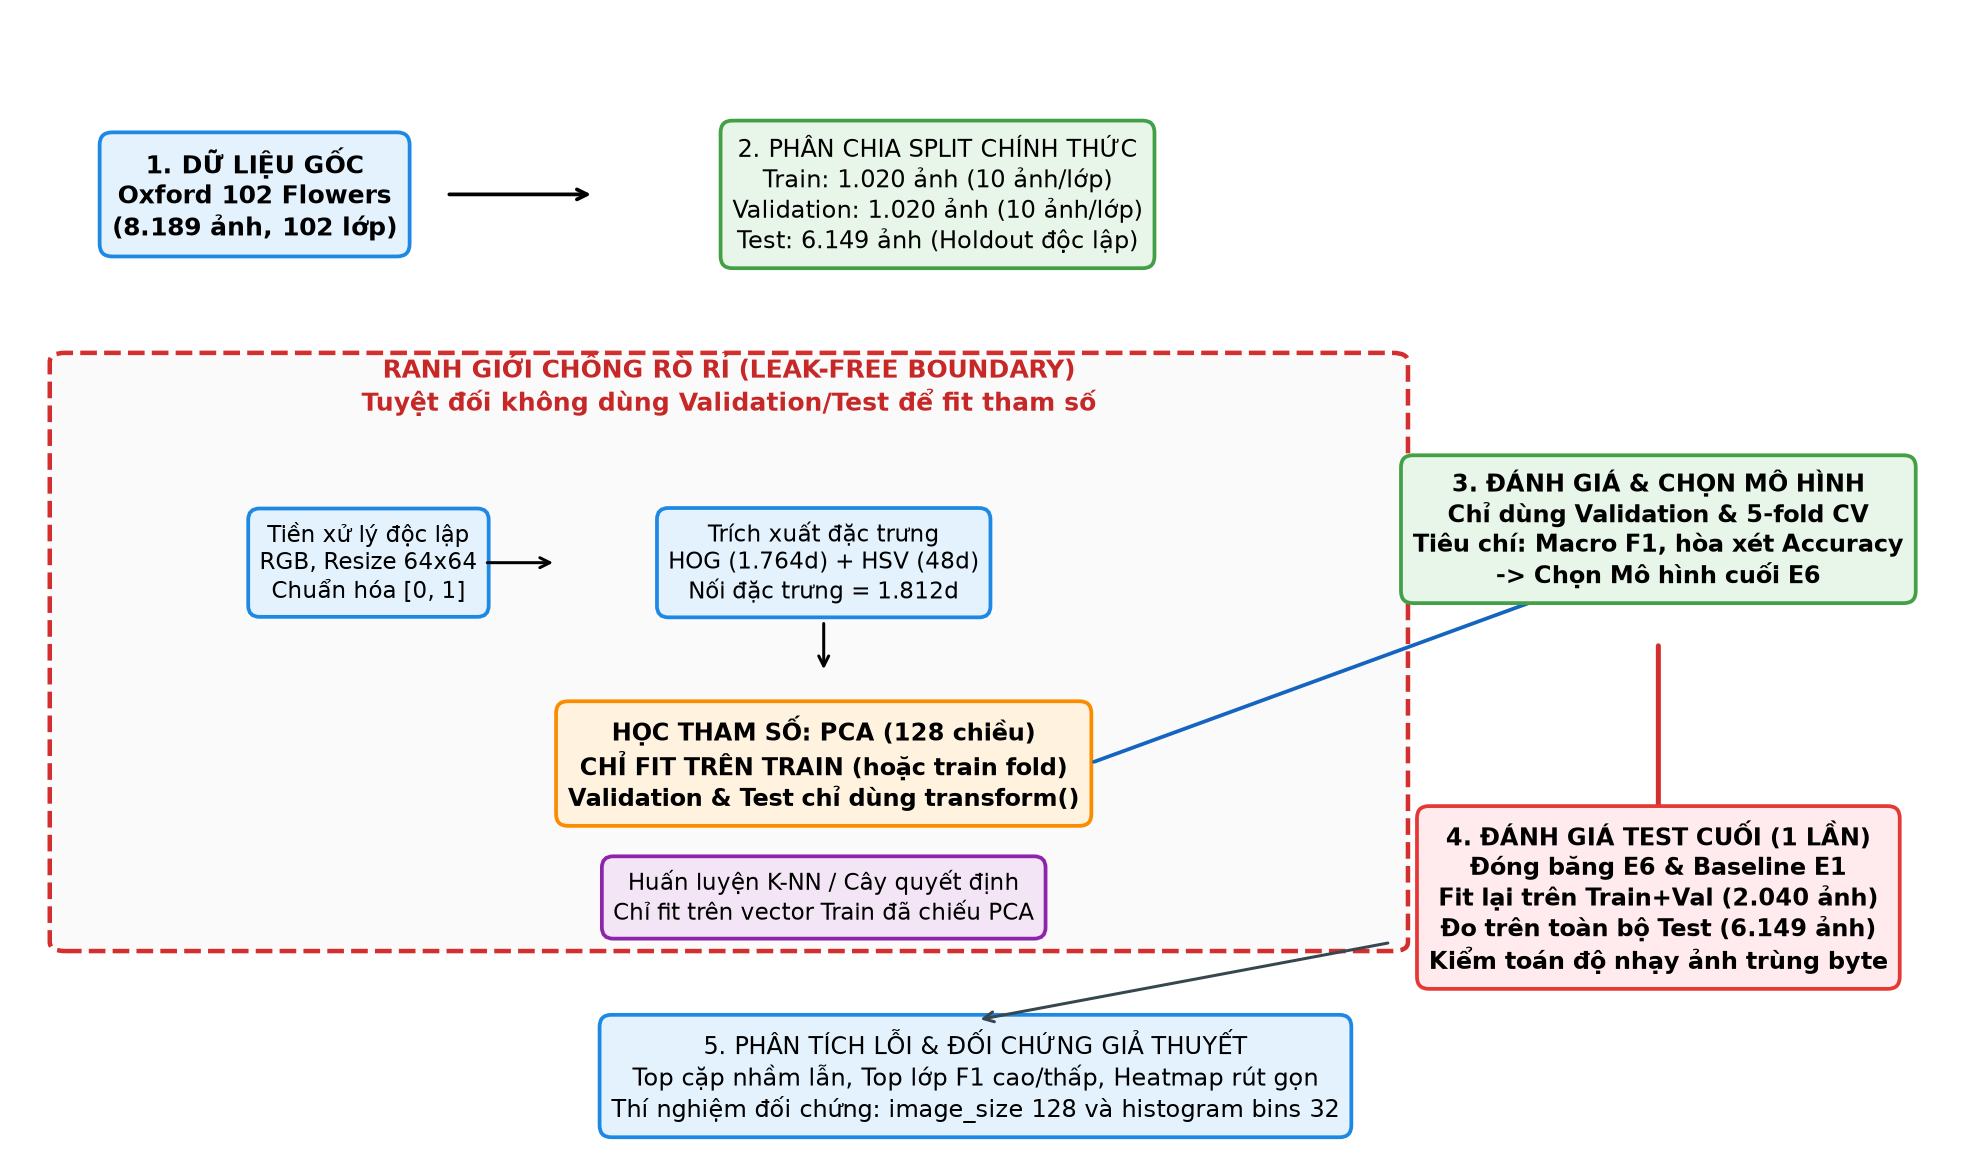
\includegraphics[width=0.95\textwidth]{figures/pipeline_sodo.png}\caption{Sơ đồ luồng xử lý tổng thể và ranh giới chống rò rỉ dữ liệu.}\label{fig:pipelinesodo}\end{figure}

Các ID ảnh trong metadata được dùng để ghép ảnh, nhãn và split. Nhóm kiểm tra các ID không bị lặp giữa train, validation và test. Với các đặc trưng tính riêng trên từng ảnh, việc trích xuất không học thống kê từ các ảnh khác. Riêng PCA phải được fit chỉ từ các vector train; trong kiểm định chéo, PCA được fit lại trong phần train của từng fold.
\section{Tiền xử lý ảnh}
Ảnh được chuyển về RGB, resize về 64×64 bằng nội suy song tuyến tính rồi chia giá trị pixel cho 255 để đưa về khoảng [0, 1]. Nhờ đó, mỗi ảnh có kích thước và miền giá trị thống nhất trước khi đưa vào thuật toán. Cách resize vuông khá đơn giản nhưng có thể làm thay đổi tỉ lệ hình dạng; nhóm xem đây là một hạn chế của phương pháp.

Nhóm dùng cùng mã tiền xử lý cho huấn luyện và suy luận. Việc này quan trọng vì nếu ảnh dự đoán được xử lý khác ảnh train thì khoảng cách giữa các vector có thể thay đổi, khiến kết quả không phản ánh đúng mô hình đã huấn luyện.
\section{Các đặc trưng sử dụng}
\textbf{Pixel:} Sau khi resize, ba kênh màu được trải thành vector 64×64×3, tương ứng 12.288 giá trị. Cách này giữ lại thông tin màu và vị trí tương đối của pixel, nhưng nhạy với sự thay đổi vị trí hoa, nền và ánh sáng.

\textbf{HOG:} Histogram gradient có hướng mô tả hướng thay đổi cường độ sáng trong từng vùng ảnh \cite{hog}. Với cấu hình V1 gồm 9 hướng, ô 8×8 và khối 2×2, một ảnh tạo ra 1.764 đặc trưng HOG. Ảnh được chuyển sang xám trước khi tính HOG, vì vậy đặc trưng này giữ thông tin biên nhưng bỏ thông tin màu.

\textbf{HOG kết hợp HSV:} Nhóm bổ sung histogram màu HSV gồm 16 bin cho mỗi kênh. HOG và histogram được chuẩn hóa L2 riêng rồi nối lại, tạo 1.812 đặc trưng ở cấu hình ô 8×8. Mục đích là giữ thông tin cạnh từ HOG đồng thời bổ sung đặc điểm màu của ảnh. Histogram không phân biệt vị trí màu nên cũng có thể bị ảnh hưởng bởi màu của nền.

\textbf{PCA:} Phân tích thành phần chính tạo không gian có số chiều thấp hơn dựa trên phương sai của các vector train. Nhóm dùng PCA randomized với 128 thành phần; cấu hình 64 chiều lấy 64 thành phần đầu của cùng phép fit 128 chiều. PCA được học riêng trên train, không fit trên validation hoặc test. Việc giảm chiều có thể giảm chi phí tính khoảng cách nhưng cũng có thể làm mất thông tin hữu ích cho phân loại.
\section{Mô hình và chỉ số đánh giá}
K-NN tìm các mẫu train gần ảnh cần dự đoán rồi dựa vào nhãn của các láng giềng đó. Các cấu hình trong báo cáo sử dụng những giá trị $k$, khoảng cách và cách gán trọng số được ghi trong tệp cấu hình. Cây quyết định chia dữ liệu theo các ngưỡng đặc trưng; nhóm thử các độ sâu và số mẫu tối thiểu ở nút lá. Việc so sánh hai mô hình giúp nhóm thấy ảnh hưởng của cả cách biểu diễn ảnh và cách phân loại.

Accuracy là tỉ lệ dự đoán đúng trên toàn bộ mẫu. Precision của một lớp thể hiện tỉ lệ dự đoán thuộc lớp đó là đúng; Recall thể hiện tỉ lệ mẫu thật của lớp được nhận đúng. F1 là trung bình điều hòa của Precision và Recall. F1 trung bình vĩ mô lấy trung bình F1 của 102 lớp với trọng số bằng nhau; chỉ số có trọng số lấy theo số mẫu từng lớp. Nhóm ưu tiên F1 vĩ mô khi chọn mô hình để không chỉ dựa vào các lớp có nhiều ảnh. Điểm bỏ phiếu K-NN không được coi là xác suất đã hiệu chuẩn.
\section{Cách tính khoảng cách và bỏ phiếu của K-NN}
Với một ảnh cần dự đoán, K-NN so sánh vector đặc trưng của ảnh đó với các vector trong tập train. Ở khoảng cách Euclidean, khoảng cách giữa hai vector $x$ và $y$ được tính bằng $d(x,y)=\sqrt{\sum_i(x_i-y_i)^2}$. Nếu hai ảnh gần nhau theo cách đo này, chúng có khả năng được đưa vào danh sách láng giềng của nhau. Tuy nhiên, ảnh gần nhau trong không gian đặc trưng không nhất thiết cùng loài, vì đặc trưng có thể giữ cả thông tin nền hoặc ánh sáng.

Khoảng cách cosine dựa trên góc giữa hai vector, thay vì chỉ nhìn độ lớn chênh lệch từng phần tử. Sau khi chọn $k$ láng giềng, mô hình có thể cho mỗi láng giềng trọng số bằng nhau hoặc ưu tiên láng giềng gần hơn. E6 dùng $k=3$, cosine và trọng số theo khoảng cách. Nhóm em không diễn giải trọng số bỏ phiếu này như độ tin cậy đã hiệu chuẩn vì chưa thực hiện kiểm định hiệu chuẩn xác suất.

Việc chọn $k$ có đánh đổi. Giá trị nhỏ dễ phụ thuộc vào một vài mẫu gần nhất; giá trị lớn hơn tổng hợp nhiều mẫu hơn nhưng có thể đưa các lớp khác vào cùng lượt bỏ phiếu. Với dữ liệu chỉ có 10 ảnh train mỗi lớp, sự khác biệt giữa các lựa chọn này có thể khá rõ. Nhóm chỉ thử tập cấu hình đã định trong file YAML và chọn bằng validation; không điều chỉnh tiếp bằng test.
\section{Chuẩn hóa khối và giảm chiều}
Vector HOG và histogram màu có số chiều và thang giá trị khác nhau. Nếu chỉ nối hai vector mà không kiểm tra thang đo, một khối có thể chi phối phép tính khoảng cách. Vì vậy, ở E4 và E6 nhóm chuẩn hóa L2 từng khối trước khi nối. Sau bước này, hai khối có trọng lượng tổng thể bằng nhau theo cách tính hiện tại. Đây là một lựa chọn thiết kế để dễ so sánh, không phải bằng chứng rằng trọng số bằng nhau là tối ưu cho mọi ảnh.

PCA tìm các hướng biến thiên từ dữ liệu được đưa vào khi fit. Nếu PCA được fit bằng cả train và validation thì phân bố validation đã ảnh hưởng đến phép biến đổi, dù nhãn validation không được dùng ở bước đó. Nhóm tránh điều này bằng cách fit PCA sau khi đã tách train. Trong kiểm định chéo hoặc đường học, PCA được fit lại trên đúng phần train hoặc tập con train tương ứng của từng lần thử.

Đối với các cấu hình 64 và 128 chiều của V2, nhóm dùng một phép fit randomized PCA 128 chiều trên train rồi lấy 64 thành phần đầu cho cấu hình nhỏ hơn. Cách làm này tiết kiệm phép tính và đã được ghi rõ trong cấu hình; kết quả không nhất thiết giống hoàn toàn việc fit riêng một PCA randomized 64 chiều.
\section{Ý nghĩa của ma trận nhầm lẫn}
Ma trận nhầm lẫn đặt nhãn thật theo một chiều và nhãn dự đoán theo chiều còn lại. Các ô trên đường chéo cho biết số mẫu được nhận đúng; ô ngoài đường chéo cho biết số lần một lớp bị dự đoán thành lớp khác. Chẳng hạn, một cặp 24 đến 11 có hướng: số ảnh lớp thật 24 được dự đoán là 11, không tự động bằng số ảnh lớp thật 11 được dự đoán là 24.

Với 102 lớp, một hình ma trận đầy đủ khó quan sát từng ô. Vì vậy nhóm lưu thêm bảng các cặp nhầm và ví dụ ảnh. Việc xem ảnh giúp đặt câu hỏi về màu sắc hoặc bố cục, nhưng cần có phép thử kiểm soát trước khi kết luận yếu tố đó thực sự gây ra lỗi.
